\documentclass[MasterNotes.tex]{subfiles}
\begin{document}
	
\begin{frame}
	\frametitle{Survival Analysis with Python}
	\large
\begin{figure}
\centering
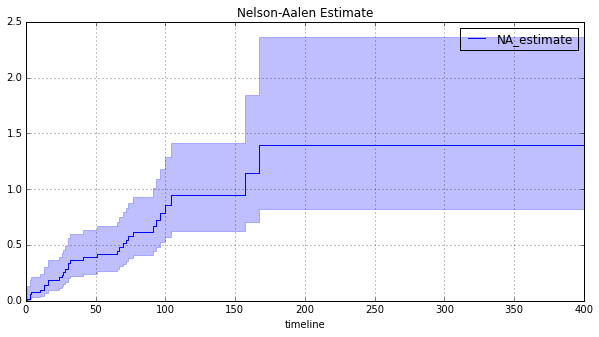
\includegraphics[width=0.99\linewidth]{images/lifelines-plotly-NAFplot}
\caption{}
\label{fig:lifelines-plotly-NAFplot}
\end{figure}
\end{frame}

\begin{frame}
	\frametitle{Survival Analysis with Python}
	\large
\begin{figure}
\centering

\includegraphics[width=0.99\linewidth]{images/lifelines-logo}
\caption{}
\label{fig:lifelines-logo}
\end{figure}
\end{frame}
%=================================================%	
\begin{frame}
\frametitle{Survival Analysis with Python}
\large	

\begin{figure}
\centering
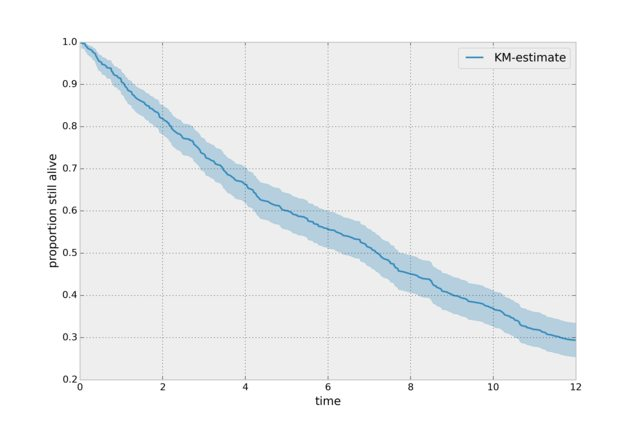
\includegraphics[width=0.97\linewidth]{images/lifelines-kmplot}
\caption{}
\label{fig:lifelines-kmplot}
\end{figure}
\end{frame}
%================================================%
\begin{frame}[fragile]
\frametitle{Survival Analysis with Python}
\large	
\begin{figure}
\centering
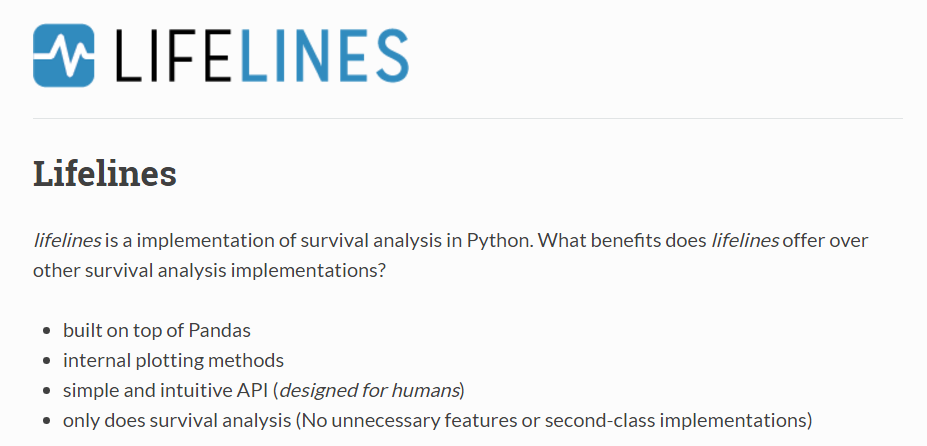
\includegraphics[width=0.7\linewidth]{images/LifeLines-Screenshot}
\caption{}
\label{fig:LifeLines-Screenshot}
\end{figure}





\end{frame}


\end{document}	